\section{Introduction}
\label{sec:introduction}
Generating collision-free trajectories when dealing with multiagent systems is a safety-critical task. In missions that require cooperation of multiple agents, such as surveillance \cite{vallejo2009multi}, crop inspection \cite{carbone2018swarm} and warehouse management \cite{guizzo2008three}, it is often desirable to safely drive the agents from their current locations to a set of final positions. Solving this problem, known as multiagent point-to-point transitions, is therefore an integral objective of any robust multiagent system.

There are two main variations of the multiagent point-to-point transition problem: the labelled or the unlabelled agent problems. In the former, each agent has a fixed final position that cannot be exchanged with other agents \cite{schouwenaars2001mixed, augugliaro2012generation}; in the latter, the algorithm is free to assign the goals to the agents, as to ease the complexity of the trajectories \cite{turpin2012decentralized}. This paper will focus on the labelled agent version. 

A common approach is to formulate an optimization problem. One of the first techniques developed relied on Mixed Integer Linear Programming (MILP), modelling collision constraints as binary variables \cite{schouwenaars2001mixed}. These methods, although viable, are computationally heavy and not suited for large teams.

More recently, Sequential Convex Programming (SCP) \cite{boyd2008sequential} has been used for faster computation compared to MILP. In \cite{augugliaro2012generation}, SCP is used to compute optimal-fuel trajectories of quadrotor teams. A decoupled version of that algorithm (dec-iSCP) is proposed in \cite{chen2015decoupled}, which has shorter computation time at the cost of suboptimal solutions. However, dec-iSCP is a sequentially greedy approach that makes the optimization problem harder to solve as more vehicles are added.

Discrete approaches divide the space in a grid and use known discrete seach algorithms \cite{preiss}. Other mixed approaches combine optimization techniques and predefined behaviours to manage collisions \cite{tang2018complete}. Lyapunov barrier functions have also been used to compute multiagent collision-free trajectories \cite{wang2017safety}.

Distributed optimization approaches can effectively include pair-wise distance nonlinear constraints \cite{bhattacharya2011distributed}. Furthermore, the distributed nature reduces the computational effort with respect to centralized approaches. A new solution to the problem is proposed in this paper, based on distributed model predictive control (DMPC) \cite{camponogara2002distributed}. Synchronous implementation of DMPC \cite{dai2017distributed,wang2014synthesis}, allows the agents to solve their optimization problems in parallel. Previous work on DMPC shows its capabilities in multiagent tasks, such as formation control \cite{van2017distributed,sayyaadi2017decentralized}, but not explicitly for point-to-point transitions as highlighted in Fig.~(\ref{fig:30_random}).

The rest of the paper is organized as follows: Section II formulates the optimization problem solved by each agent, and Section III formalizes the DMPC algorithm for multiagent point-to-point transitions. Finally, Section IV presents simulation results of DMPC and compares its performance with dec-iSCP.

\begin{figure}[t]
	\centering
	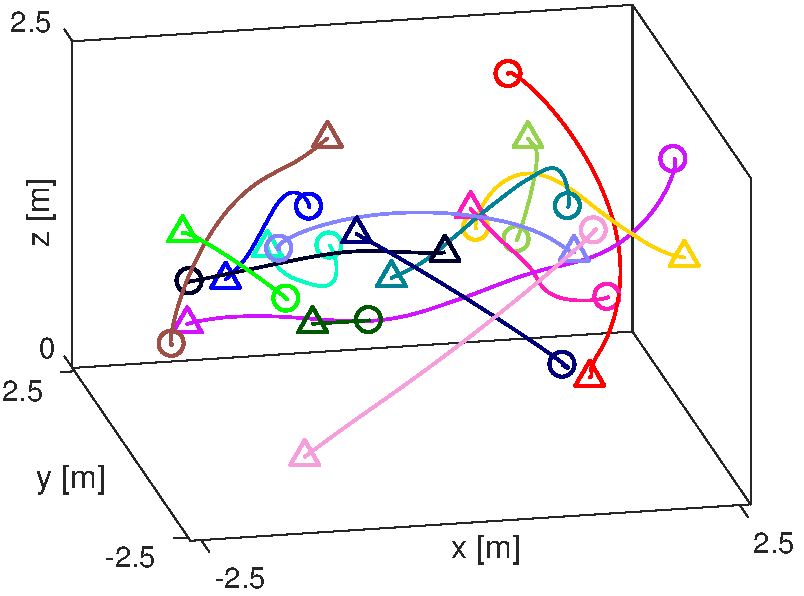
\includegraphics[width=0.45\textwidth]{figures/30_rand}
	\caption{A 15-vehicle point-to-point transition solved using our DMPC algorithm. The initial and final positions (denoted with triangles and circles, respectively) were chosen randomly within a convex volume of $5 \times 5 \times 2$m. The agents were required to maintain a minimum distance of 0.75m of each other throughout the trajectory. Even in this highly cluttered dynamic environment, the proposed algorithm is capable of quickly finding a collision-free trajectory for all agents.}
	\label{fig:30_random}
\end{figure}






